\section{Fundamentals of  Automated Planning}
\label{sec:europa}

{\footnotesize
  \begin{quote}
[Planning] \emph{is an abstract, explicit deliberation process that chooses and
organizes actions by anticipating their expected outcomes. This
deliberation aims at achieving as best as possible some prestated
objectives. Automated planning is an area of Artificial Intelligence
(AI) that studies this deliberation process computationally.} -- from
\textbf{Automated Planning Theory and Practice} by Ghallab, Nau and
Traverso \cite{ghallab04} 
\end{quote}
}

% Planning, for our purposes, can be thought of as determining all the
% small tasks that must be carried out in order to accomplish a goal.
To articulate the fundamentals of automated planning briefly and use
that to motivate the mechanisms we use in our specific form of the
technique we start with a simple example.

\begin{quotation}

  In the near future, a personal robot sets out to buy a gallon of milk
  This involves a number of tasks: obtain keys, obtain wallet,
  start car, drive to store, find and obtain milk, purchase milk, etc.
  The embedded planner has to have a ``model'' of the world in which it
  lives and has to use the task primitives in this model to structure
  the actions so it achieves its goal. Constraints control when certain
  tasks can or cannot occur. For example the robot must obtain the keys
  and wallet \emph{before} driving to the store and pick up the milk
  \emph{before} purchasing it.

\end{quotation}

For such a robot the milk buying plan at the store might look like
\comment{Figure needed}.


% \eu is a general purpose AI planning toolkit developed at NASA Ames.  
% TODO: Talk about NASA missions where \eu has been used.

\eu is a versatile planning framework which can be used in a range of
problem-solving methods. 

\paragraph \texttt{Constraint Satisfaction}: A canonical problem in
dealing with constraints is the $N$-Queens problem in which chess queens
must be placed on an  $N$x$N$ chessboard so no queens attack the other. Fig.
\ref{fig:nqueens-1} shows an example of a random positioning of queens
on a  $N$x$N$ chessboard. Queens in violation of the non-attack constraint
are highlighted in red.

\begin{figure} \centering
  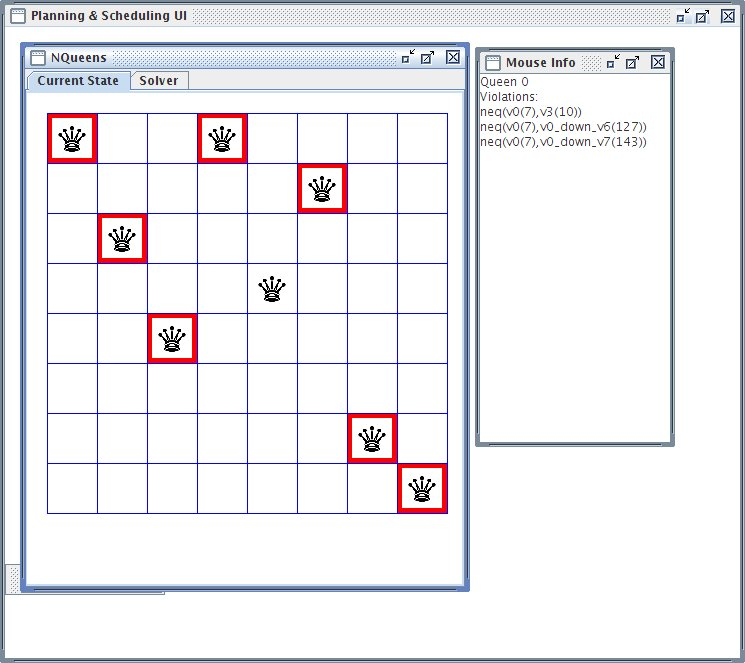
\includegraphics[scale=0.35]{figs/Example-NQueens0.jpg}
  \caption{\small N-Queens problem. Queens in violation of the
    non-attack constraint are highlighted in red.}
\label{fig:nqueens-1}
\vskip+0.1cm
\end{figure}


If we define $N$x$N$ variables Q$_{rc}$, $r \in [1,N]$, $c \in [1,N]$,
Q$_{rc} = 1$ if cell $r,c$ in the chessboard is occupied by a Queen, $0$
otherwise. Then the following constraints need to be satisfied:

\begin{equation}
 Sum(Q_{rc})= \left\{
\begin{array}{l l}
  1 & \forall r \quad \mbox{(only one Queen per row)}\\
  1 & \forall c \quad \mbox{(only one Queen per column)}\\ 
\end{array} \right.
Sum(Q_{r+i,c+i}) = 1\\
Sum(Q_{r-1,c+i}) = 1 \quad \mbox{(only one Queen on each diagonal)}\\
\end {equation} 

\comment{fix \newline and numbering problem above}

The problem can be solved by finding assignments for all variables
Q$_{rc}$ that satisfy the above constraints. Fig. \ref{fig:nqueens-2} is
a solution found by \eu using that formulation and a specialized search
procedure.

\begin{figure}
\centering
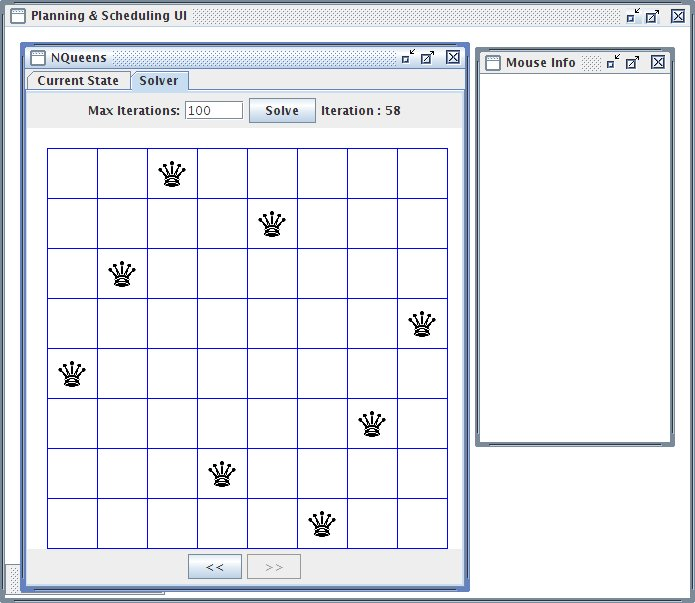
\includegraphics[scale=0.35]{figs/Example-NQueens1.jpg}
\caption{\small N-Queens solution generated by \eu}
\label{fig:nqueens-2}
\vskip+0.1cm
\end{figure}


\paragraph \texttt{Scheduling}: In the Resource Constrained Project
Scheduling Problem (RCPSP), a project consisting of a set of activities
must be scheduled in a way that satisfies minimum and/or maximum
temporal separation constraints. The activity schedule must also respect
fixed limits on the availability of resources required to perform each
activity. In addition to satisfying temporal and resource constraints,
it is common for the user to want to minimize makespan so that the
entire project is finished as early as possible. Fig. \ref{fig:rcpsp-1}
shows an example of a a solution provided by \eu for an RCPSP instance
with 10 activities, 5 resources and 30 temporal constraints.

\begin{figure}
\centering
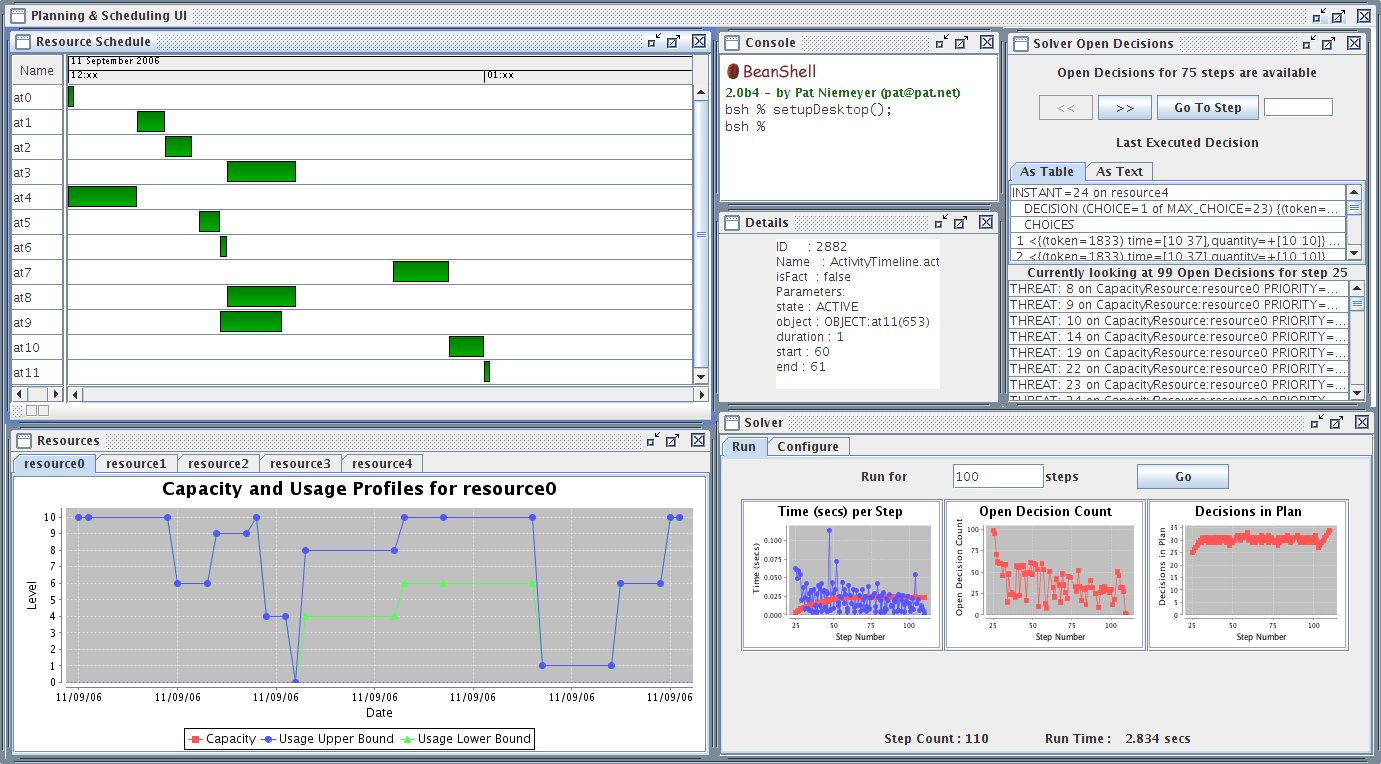
\includegraphics[scale=0.35]{figs/Example-UBO0.jpg}
\caption{\small RCPSP problem}
\label{fig:rcpsp-1}
\vskip+0.1cm
\end{figure}


\paragraph \texttt{Planning}: In the Shopping Agent Problem
\cite{russelnorvig} an agent needs to purchase a set of products (milk,
drill, etc) that are available at specific locations (supermarket,
hardware store, etc), the agent is subject to temporal (must complete
tasks by specific deadlines) and resource (fuel, carrying capacity, etc)
constraints. The agent must figure out what actions need to be performed
to find and acquire the required items, as well as when to perform each
of those actions.

Below is a solution produced by \eu for a simple problem instance where
the shopping agent needs to buy Bananas, Milk and a Drill.

\begin{figure}
\centering
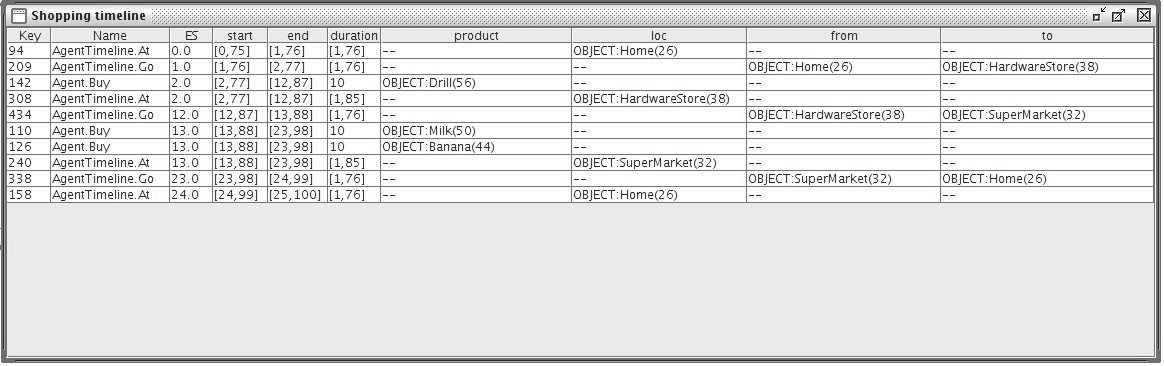
\includegraphics[scale=0.35]{figs/Example-Shopping0.jpg}
\caption{\small Shopping Agent problem}
\label{fig:shopping-1}
\vskip+0.1cm
\end{figure}


As we can see, a planning problem (what actions must be performed to
achieve a goal) may embed a scheduling problem (in what order should
those actions be performed), and both planning and scheduling embed
Constraint Satisfaction problems since temporal, resource and many other
kinds of constraints must be respected in most real life problems.

These relationships between Planning, Scheduling and Constraint
Satisfaction have been examined in detail in the literature (TODOL ref
Frank et al on Planning vs. Scheduling), and they lead to \eu's use of
constraint reasoning as its innermost building block. Below we examine
the main ideas from Constraint Satisfaction Programming, and from
Constraint Based Planning and Scheduling that constitute \eu's
theoretical underpinnings, then we dive into how \eu implements those
ideas.

\subsection{Constraint Programming}
\label{sec:europa:cp}

Constraint Satisfaction Programming, also know as Constraint Programming (CP) is a discipline that provides a generic framework for representing, solving and making logical inference on constraints. A complete treatment of this discipline is given in [MAR98] and [APT03] and very concise introductions are provided in [BAR99] and [LUS01]. 

	A constraint programming problem consists of a set of variables V={x1,..,xN}, where each variable takes values from a domain d1,..,dN. Domains are most often discrete and finite, but there are numerous CP implementations associated with continuous domains. Given a defined conjunctive set of constraints on the variables: $C=\{c1(x1,..,xN), ..., cK(x1,..,xN)\}$, the objective is to find one or more value assignments to V where all constraints are satisfied.

To solve a problem, CP uses logical inference to perform 2 operations:

\begin{enumerate}
	\item Bounds propagation: To infer upper and lower variable bounds. For example, from the constraints x1 + x2 <= 2, xi>=0, we can infer [0,2] bounds for x1 and x2

	\item Domain reduction: To infer a valid set of values for a variable. For example, for discrete variables, the constraints allDifferent(x1,x2,x3) and xi>=0, xi <=4. if x1 =1 and x2=3 we can infer that the valid domain for x3 is reduced to {2,4} 

\end{enumerate}

CP is normally implemented as part of a programming language and constraints are normally represented as objects [PUG95]. Any constraint can be introduced and, as long as the bounds propagation and domain reduction protocols specified by the host CP system are enforced, it will be indistinguishable from any other ÒprimitiveÓ CP constraint, such as <= or >=.

Solving a CSP is NP-Hard in theory, but often very efficient in practice using a number of algorithms and techniques that are well understood.

TODO: talk about arc consistency algorithms, computational complexity and solvers.


\subsection{Constraint-Based Attribute and Interval Planning}
\label{sec:europa:cp}


The most common planning formulations use a propositional representation, where the state of the world is represented by a set of propositions (statements that can be true or false), and operators change the truth values of these propositions (TODO ref?). Although these formulations are powerful and have allowed researchers to develop numerous contributions in automated planning, there are many classes of problem domains that are difficult it is difficult to represent using them. 

In particular, it is hard to represent time, resources, mutual exclusion and concurrency using propositions (TODO: ref?).  It is straightforward to represent and reason about all of those elements using a CSP representation, as a result there has been some work on doing automated planning while taking advantage of CSP  (TODO: ref).  Traditionally, the entire planning problem is translated into a CSP and then solved using traditional CSP methods, this leads to a formulation where action choices and relationships are represented as variables and/or constraints. However, this has at least two major drawbacks:
\begin{enumerate}
	\item Given that action choices and relationships (rules) are expresed through variables, the domain descriptions that result from this approach are not intuitive and therefore difficult to understand and debug
	\item If the structure of a planning model (actions, conditions, effects, dependencies at the action level, etc) is not explicitly maintained by the CSP planner, the search algorithms are deprived of critical information to make better decisions. If that structure is maintained somehow (for instance, by internally marking variables that represent action choice and relationships between actions), it is still hard to write search algorithms as any planning-specific insight has to be translated into the CSP representation of variables and constraints  (TODO: example?)
\end{enumerate}


Constraint-Based Attribute and Interval planning (CAIP) (TODO:ref) is intended to close that gap: on the one hand, it takes advantage of a CSP representation, but it also uses attributes and intervals to maintain an explicit representation of the elements relevant to planning, so that it is easier to write algorithms that search for an reason abut plans. The main elements of CAIP are:

\begin{enumerate}
	\item Intervals:
	\item Attributes:
	\item Domain Constraints an Configuration rules:
\end{enumerate}

TODO: Explain how planning problem instances and their solutions are represented.

